\documentclass[a4paper,11pt,fleqn]{jbook}
%\documentclass[a4paper,11pt]{jarticle}
%\usepackage{u-thesis}
\usepackage{u-thesis-p}
\usepackage{graphicx}
\usepackage{amsmath}
\usepackage{mediabb}%pdf

\usepackage{ascmac}
\usepackage{here}
\usepackage{txfonts}
\usepackage{listings,jlisting}


% title
\title{LLVMコンパイラ基盤を用いた}
\titletwo{ベクトル化コード生成についての検討}
\author{永池 晃太朗}
\kind{卒業論文}  % 卒業論文
\date{2022年3月}
\lab{宇都宮大学工学部}
\labtwo{情報工学科}
\id{XX-XX}  % 学科から指定された番号をいれる

\etitle{Consideration of Automatic Generation of Vectorized Code}
\etitletwo{Using LLVM Compiler Infrastructure}
\eauthor{Kotaro Nagaike}

\begin{document}

\maketitle

\begin{jabstract}
従来のSIMD命令では同時演算数を変更する場合,それに応じて機械語コードを作り直す手間があった.
そこで,データ並列処理のために機械語コードの変更なく,同時演算数を変更できるスケーラブルなベクトル拡張を実現したベクトル拡張付きRISC-Vが開発された.ベクトル拡張付きRISC-Vではプレディケートレジスタを用いたベクトル処理を行うことによってスケーラブルなベクトル拡張を実現している.
しかし,このベクトル拡張に対応したコンパイラがないため,ベクトル拡張付きRISC-Vのアセンブリコードを生成できないという問題点がある.これに対する解決策としてベクトル拡張付きRISC-Vに対応したコンパイラの開発を検討した.コンパイラ基盤であるLLVMを用いて既に実装済みのRISC-V向けコンパイラの機能を再利用すればコンパイラを一から開発するより容易にアセンブリコードの生成を行うことができる.また,LLVMの機能である自動ベクトル化を用いることでベクトル化されたコードの生成が可能であることから,LLVMを用いることによってベクトル拡張付きRISC-V向けにアセンブリコードを得ることができると考えた.

本論文ではLLVMコンパイラ基盤におけるコード生成について述べ,そのコード生成において用いられる命令の定義手法から,独自命令生成のための命令定義を行った.独自命令の定義として命令フォーマット,出力する命令ニーモニックについて定義を行う.そして,ベクトル化されたLLVM中間表現であるLLVM IRから独自命令の生成を可能としている.

本論文ではベクトル拡張付きRISC-Vの命令の内,ベクトル算術・論理演算命令,即値を用いるシフト命令の実装について述べる.

更に,実装した命令が正常に入力ソースコードから生成されることを確認する.C言語を用いて配列加算等のプログラムを作成し,そのプログラムのアセンブリコードの生成を行う.

また,現段階では実装できていない命令として,ベクトルロード・ストア命令等がある.その命令生成に向けて新たに必要な定義や変更点などについて述べる.
\end{jabstract}

%abstract
\begin{abstract}
For processing that performs the same operation on multiple data, such as image processing, it is possible to achieve higher speed by using data parallel processing with SIMD instructions that process multiple data with a single instruction.
However, when using SIMD for data parallel processing, the number of simultaneous operations, which is the number of data to be processed in one instruction, is fixed for SIMD instructions. Therefore, if the number of concurrent operations is changed in order to increase the processing performance, the machine language code must be rewritten.
To solve this problem, RISC-V with vector extension has been developed to realize scalable vector extension that can change the number of concurrent operations without changing the machine code.

However, there is a problem that the assembly code of RISC-V with vector extension cannot be generated because there is no compiler that supports this vector extension. As a solution to this problem, I consider how to realize a compiler that supports RISC-V with vector extensions. By using LLVM, which is a compiler infrastructure, and reusing the functions of already implemented compilers for RISC-V, it is easier to generate assembly code than developing a compiler from scratch. In addition, the automatic vectorization function of LLVM can be used to generate vectorized code, so I consider that assembly code for RISC-V with vector extensions can be obtained by using LLVM.

In this paper, I describe the code generation in the LLVM compiler infrastructure and define instructions for generating original instructions. Among the instructions of RISC-V with vector extensions, I describe the implementation of vector arithmetic and logic instructions and shift instructions using immediate values.
In addition, I confirm that the implemented instructions can be successfully generated from the input source code, and show that programs such as array addition written in C can be used to generate their vectorized assembly code.
I will also show that the vectorized assembly code can be generated using programs such as array addition written in C. There are instructions such as vector load/store instructions that have not been implemented at this stage. In this paper, I describe the definitions and changes required to generate such instructions.    % 同一ディレクトリのabstract.texが読み込まれる
\end{abstract}

\newpage
\tableofcontents    % 目次


\newpage
\chapter{はじめに}
\label{chp:intro}   % ラベルを貼っておくと後々便利
%intro.tex
FPGA(Field Programmable Gate Array)はユーザによって回路の再構成が可能なLSIであり,目的の処理をハードウェアとして実装可能なデバイスである.
近年FPGAの大容量化,高性能化によって大規模な回路が実現可能になった.これによりFPGAは自動運転を始めとする組込み分野での利用増加が期待されている.

FPGAを用いたハードウェア開発はHDL(Hardware Description Language)によるRTL(Register Transfer Level)設計が広く用いられている.RTLはFPGA上に構成する回路の信号の流れや制御構造を直接設計できる一方,動作検証やデバックが難しく,短期間で複雑な処理の開発は困難である.\cite{bib:fpga}
そのため,FPGAによる開発期間を短縮する方法として,専用ハードディスクとプロセッサを用いたソフトウェアによる処理を組み合わせる方法が考えられる.FPGA上のハードウェアリソースを用いて実装するプロセッサのことをソフトコアプロセッサという.
一般的に組込みシステムではそのコストやサイズ,消費電力などに制限があるためハードウェア資源に制約があることが多く,メモリバンド幅が限られることからメモリシステムの性能が高くないことが多い.メモリシステムの性能が低いと演算性能を高くしてもメモリアクセスに時間がかかり,結果としてシステム全体の性能はメモリシステムの性能によって左右される.\cite{bib:2}
そこで,ソフトコアプロセッサによる処理を考える.すべての処理を専用ハードウェア回路で行うのではなく,高い性能の求められない汎用的な処理についてはソフトコアプロセッサにて行うことにより開発する専用ハードウェア回路を削減でき,ソフトコアプロセッサの性能が向上して専用ハードウェア回路を削減しても求められた性能に達することができればハードウェアの開発コストを抑えることができる.

組込み分野ではAI技術に注目が集まっている.独立行政法人情報処理推進機構の調査によると,将来強化/新たに獲得したい技術として組込み/IoT関連企業の46\%がAI技術を挙げている.\cite{bib:ipa}

AI技術の応用としては画像認識などの画像処理が行われる.画像処理では画像を構成する画素に対して同じ処理を行うようなものが多い.このように複数のデータに対して同じ演算を行う処理については,単一命令で複数データの処理を行うSIMD(Single Instruction, Multiple Data)や,複数命令を並列に実行するMIMD(Multiple Instruction, Multiple Data)による並列処理で高速化が可能である.\cite{bib:simd,mimd}
MIMDは複数の制御を並列化することができるため,異なる処理を同時に実行するアプリケーションでは有効である.しかし,プロセッサに複数の制御ユニットをもたせる必要があるためSIMDと比較するとハードウェアのコストが大きくなる.一方SIMDは単一の制御ユニットで複数の演算ユニットを並列動作させるため制御ユニットのコストは低くなる.
データ並列処理では複数のデータに対して同じ処理を実行するためSIMDによって並列処理が可能である.

SIMDによる並列処理を行う場合,SIMD命令は1命令で演算するデータ数が決まっている.そのため演算性能を上げるために同時演算数を変更すると機械語コードを作り直す必要がある.異なる同時演算数でも同一の機械語コードを利用可能とするためには,機械語コードが同時演算数に依存しないスケーラブルなベクトル拡張が必要である.スケーラブルなベクトル拡張により機械語コードを変更することなく,必要に応じて容易に同時演算数を増やし高性能化することが可能となる.

スケーラブルなベクトル拡張を実現したものとしてオープンな命令セットアーキテクチャであるRISC-V\cite{bib:risc-v}をベクトル拡張したベクトル拡張付きRISC-V\cite{bib:kimura}が提案されている.ベクトル拡張付きRISC-Vは組込み機器に広く用いられているARMのベクトル拡張であるARM SVE(Scalable Vector Extension)\cite{bib:arm_sve}の命令セットを参考に組み込み向けにRISC-Vに拡張したものである.しかし,ベクトル拡張付きRISC-Vに対応したコンパイラが存在していない.そこで解決策としてベクトル拡張付きRISC-Vのベクトル命令のアセンブリコードを得るためのコンパイラの開発を検討した.

本論文では,第2章で現在のMIQSプロセッサについて述べる.第3章でベクトル拡張付きRISC-V命令の生成のために利用したコンパイラ基盤であるLLVMについて述べる.第4章で実際に命令生成のための実装について述べる.第5章では実際のソースコードからアセンブリコードの出力を行った結果について述べる.


\newpage
\chapter{MIQSプロセッサ}
\label{chp:2}
%2.tex

本章ではSIMD演算機能を持つソフトコアプロセッサであるMIQSプロセッサについて述べる.


\section{RISC-V}
\label{chp:2_1}
%2.1.tex

RISC-Vはカルフォルニア大学バークレイ校が新たに開発したRISCの設計思想に基づく命令セットアーキテクチャ(ISA)である.RISC-VはオープンなISAであり,ライセンスが不要である.

従来のISAでは,後方バイナリ互換性を維持するために過去に拡張した命令すべてを実装する必要がある.しかし,このようなISAでは命令数が増加し複雑になる.そこでRISC-Vではモジュール式ISAを採用している.%参考文献入れる
RISC-Vのシステムの機能を独立したモジュールとして分け,アプリケーションに応じて拡張機能を組み込むかを選択できる.RISC-Vには必ず組み込まなければならない基本命令セット(RV32I)の他に,主な拡張機能として乗算及び除算(RV32M),単精度浮動小数点(RV32F),倍精度浮動小数点(RV32D)等がある.

%RISC-Vの命令フォーマットの話をする
\section{MIQS概要}
\label{chp:2_2}
%2.2.tex
ベクトル拡張付きRISC-Vプロセッサとは,RISC-Vコアにベクトル演算機能を拡張したソフトコアプロセッサである.
図\ref{fig:MIQS_system}
にベクトル拡張付きRISC-Vプロセッサの全体構成を示す.ベクトル拡張付きRISC-VプロセッサのRISC-VコアプロセッサはRISC-Vプロセッサを使用している.このプロセッサはVerilog-HDLで記述された5段パイプラインプロセッサで必要最低限の基本命令セットであるRV32Iで規定された命令を実装している.

\begin{figure}[b]
\begin{center}
    \includegraphics[scale=1.2]{image/MIQS_system.pdf}
    \caption{ベクトル拡張付きRISC-Vプロセッサの構成}
    \label{fig:MIQS_system}
\end{center}
\end{figure}

命令のフェッチおよびデコードはRISC-Vコアプロセッサ上で行い,デコード結果がベクトル拡張命令であったときはベクトル処理ユニットで動作させる.

メモリアクセスに関しては,プロセッサからメモリコントローラを介してSDRAMにアクセスする.メモリアクセス要求がプロセッサから発行されたときは,メモリコントローラがSDRAMを制御してメモリアクセスを実現する.また,ベクトルメモリアクセスに関してもメモリコントローラにて行う.
SDRAMコントローラとメモリコントローラ間のデータバス幅は128ビットであるから,プロセッサとメモリコントローラ間のデータバス幅は128ビットとなっている.

RISC-Vコアプロセッサは命令フェッチ (IF),命令デコード (ID),実行 (EX),メモリアクセス (MA),ライトバック (WB)の5段のパイプラインで構成されている.
%ベクトル処理ユニットはベクトル長を256ビット,データの型は32ビット整数型を想定して設計されている.
ベクトル処理ユニットとRISC-Vコアの双方で動作する必要のある命令に対応するためベクトル処理ユニットはRISC-Vコアと同じく5段パイプライン構成となっており,RISC-Vコアと協調動作する構成となっている.なお,命令フェッチ部分と命令デコード部分はRISC-Vコアと共通となっている.

ベクトル拡張付きRISC-Vプロセッサによってスケーラブルなベクトル拡張を実現し,同時演算数の変更によって機械語コードの変更の必要がなくなったが,ベクトル拡張付きRISC-Vプロセッサが対応している命令セットのアセンブリコード等を出力できるコンパイラがないため,C言語等のソースコードから自動でベクトル化アセンブリコードを得ることができない.
そのためコンパイラを作る必要がある.
\section{ベクトル拡張付きRISC-V}
\label{chp:2_3}
%2.3.tex

ベクトル拡張付きRISC-Vは機械語コードが同時演算数に依存しないスケーラブルなベクトル拡張を実現したISAであり,既存のRISC-VをARM SVEを参考にベクトル拡張したものである.
ベクトル拡張付きRISC-Vではスケーラブルなベクトル拡張を行うためにプレディケートによるループ制御がある.プレディケートを用いたループ処理はループカウンタと処理する全データ数を比較してループカウンタが全データ数より小さい間対応するプレディケートレジスタをTrueにする.この命令によってベクトル処理で余りの要素がある場合,余りの要素の部分に対応するプレディケートの要素のみをTrueにする.これによって余りの要素が変化してもすべてのデータ数分ベクトル処理を行うことができ,同時演算数に依存しない機械語コードが実現できる.

ベクトル命令はベクトルロード,ストア命令,ベクトル演算命令,ベクトル制御命令の3つに分けられる.RISC-Vにはカスタム命令用にオペコード領域が4つ用意されているがそのうちの2つを利用しており,1つをベクトルロード,ストア命令,もう一方をベクトル演算命令とベクトル制御命令に使用している.ベクトルロード,ストア命令のアドレスはベースとなるスカラレジスタの値にオフセットを加えることで計算する.
ベクトル演算命令は,プレディケートあり演算命令,プレディケートなし演算命令,即値による演算命令に分けられる.
浮動小数点命令は必要なハードウェア資源が多いためサポートしていない.ベクトル拡張付きRISC-Vは基本命令に関してRV32Iのみ組み込んでいる.

レジスタ構成はベクトルレジスタv0-v31,ベクトルマスク制御に用いるためのプレディケートレジスタvp0-vp7,プレディケートレジスタ同士の論理演算に用いるプレディケートレジスタvp8-vp15,RISC-Vの汎用レジスタx0-x31,プログラムカウンタとなっている.ベクトルレジスタの長さは128$\times 2^n(0\leq n\leq 4)$ビットで表され,汎用レジスタの幅は32ビットとなっている.


\newpage
\chapter{LLVM}
\label{chp:3}
%3.tex
%\ref{chp:3}章! 黙々と書こう.

本章ではベクトル命令拡張付きRISC-Vのアセンブリコードを得るためのコンパイラの開発に用いたコンパイラ基盤であるLLVMについて述べる.
\section{LLVM概要}
\label{chp:3_1}
%3.1.tex
LLVMは2000年にイリノイ大学で開発が開始されたコンパイラ基盤である.コンパイラ基盤とはコンパイラに必要となるモジュールをまとめたもので,コンパイラを開発するためのフレームワークである.
LLVMの構成を図\ref{fig:LLVM}に示す.LLVMはソースコードをLLVMの中間表現であるLLVM IRに変換するフロントエンド,LLVM IRに対して最適化等の操作やLLVM IRから機械語やアセンブリコードへの変換を行うバックエンドに分かれている.図\ref{fig:LLVM}の様に,C言語等のソースコードから任意のアーキテクチャのアセンブリコードや機械語コードの生成を行うことができる.
LLVMではこれらの機能がモジュール化されており,新規機能を実装する際に再利用することができる.例えば新たなアーキテクチャ向けのコンパイラを開発する際はバックエンドのみ実装を行い,フロントエンドについては再利用することができる.

\begin{figure}[b]
    \centering
    \includegraphics[scale=0.4]{image/LLVM.pdf}
    \caption{LLVMの構成}
    \label{fig:LLVM}
\end{figure}

LLVMには既にRISC-Vを対象としたコード生成のためのバックエンドが実装されている.本研究ではRISC-Vを独自にベクトル拡張したベクトル拡張付きRISC-Vの命令の生成を目的としているため,このRISC-V向けのバックエンドに対して変更を加えることによって独自命令コードの生成を行う.

LLVMバックエンドにおけるコード生成の流れを図\ref{fig:LLVM_backend}に示す.
LLVMバックエンドではPassによって処理が行われる.PassとはLLVMコンパイラにおいて変換や最適化を実行するもので,中間表現に対する変換や最適化等を行う.
図\ref{fig:LLVM_backend}
ではLLVMバックエンドにおけるデータフォーマットの変化と実行されるPassを表している.

\begin{figure}[tb]
    \centering
    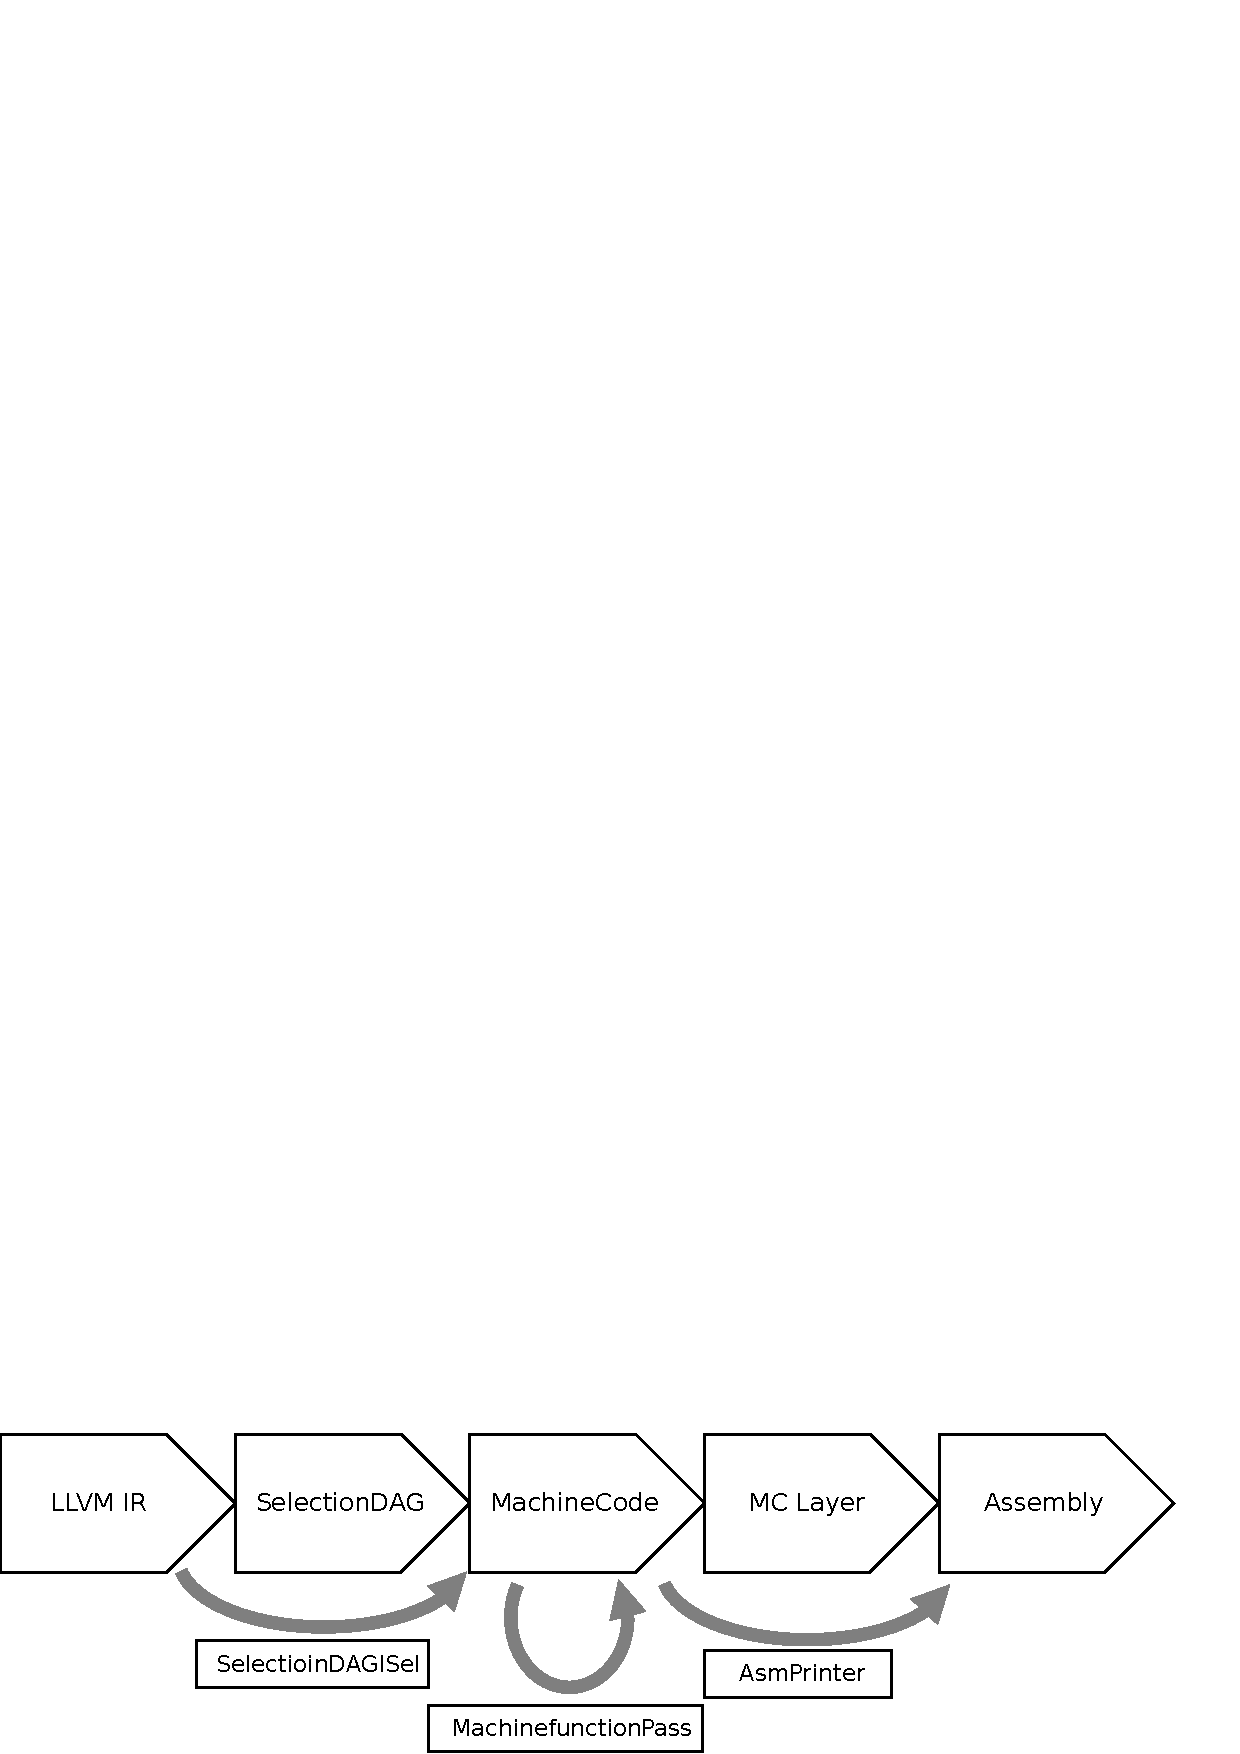
\includegraphics[scale=0.7]{image/backend.pdf}
    \caption{LLVMバックエンド}
    \label{fig:LLVM_backend}
\end{figure}

バックエンドではLLVM IRからDAG (Directed Acyclic Graph)であるSelectionDAGへフォーマットを変換する.SelectionDAGはLLVM IRをグラフ形式で表したもので,各命令やデータの依存関係を表現する.SelectionDAGへの変換はSelectionDAGISelパスで行われ,SelectionDAGは最終的にSelectionDAGISelパスによってMachineCod形式に変換される.SelectionDAGISelではLower,Combine,Legalize,Select,Scheduleのフェーズから構成される.

LowerはLLVM IRからSelectionDAGに変化させるフェーズである.このフェーズではLLVM IRからSelectionDAGのノードへと一対一の対応を行う.この段階では生成対象のアーキテクチャであるターゲットマシンでは利用できない命令やデータ形式を含んでる不正 (illegal)な状態である.

Combineフェーズではパターンマッチングによる置き換えで最適化を行い,処理に必要な命令数を削減するなどの命令の単純化を行う.

Legalizeはターゲットマシンではサポートされていない命令やデータ形式を他のものに置き換えるフェーズである.このフェーズによって不正な状態であったSelectionDAGノードがターゲットマシンで利用できない命令やデータ形式が変換され,ターゲットマシンの命令に変換が可能である正当 (legal)な状態となる.

SelectフェーズではこれまでLLVM IRの命令を用いていたSelectionDAGのノードを生成対象のアーキテクチャであるターゲットマシンの命令を用いるMachineNodeへと変換する.

Scheduleフェーズでは構築されたグラフの依存関係を元に命令をスケジューリングし,命令の順序を決定するフェーズである.

SelectionDAGISelパスではこれらのすべてのフェーズが終わった後にMachineCodeを出力する.

MachinefunctionパスではMachineCode形式をアセンブリコードや機械語コードとして出力できる様に物理レジスタの割当て等を行う.MachineCode形式はLLVM IRとは異なり,階層構造がない形式である.

MachineCodeがSelectionDAGISelによって生成された直後はまだ命令で扱うレジスタは無限個あると仮定した仮想レジスタやphi命令を含んだSSA (Static Single Assignment form)形式で表現されている.phi命令とは,SSA形式においてどの制御フローから到達したのかによって変数を選択する関数である.phi命令の例を図\ref{fig:phi_func}に示す.図\ref{fig:phi_func}ではL3で使用している変数a3の定義を決定するためにphi命令を用いている.このphi命令ではL1から来たときはa3にa1を代入し,L2から来たときはa3にa2を代入する.これによってSSA形式において変数の定義が一意に決まらない処理を実現している.
MachinefunctionPassでは仮想レジスタから実際にアセンブリコードで用いられる物理レジスタの割当てを行う.また,phi命令は従来の命令セットにおいてphi命令を実装していないためLLVMでは実行可能コード生成のためにphi命令の削除を行い,MachineCodeを非SSA形式へと変換する.

\begin{figure}
    \centering
    \includegraphics[scale=1.0]{image/phi_function.pdf}
    \caption{SSA形式でのphi命令}
    \label{fig:phi_func}
\end{figure}

AsmPrinterパスはMachineCodeをMC Layer形式へと変換した後にアセンブリコード,オブジェクトファイルを出力するパスである.MC Layer形式はMachineCode形式のような階層構造がない形式である.MC Layer形式では命令とオペランドの情報を持っており,アセンブリコードと出力する際は命令とオペランドに対応する命令ニーモニックを出力する.オブジェクトファイルを出力する際は命令とオペランドの情報をもとに対応する機械語コードを出力する.


\section{LLVMによる自動ベクトル化機能}
\label{chp:3_2}
%3.2.tex

LLVMには自動ベクトル化機能が備わっている.
自動ベクトル化とは配列の演算処理などのループによる繰り返し処理をベクトル命令の形式に置き換える機能である.LLVMによる自動ベクトル化機能はソースコードにおけるループをベクトル化されたLLVM IRへと変換が行われる.
LLVMによる自動ベクトル化の例を図\ref{fig:LLVM_auto_vec}に示す.変換元のC言語による配列加算プログラムを図\ref{fig:LLVM_auto_vec}の上に,変換後のベクトル化されたLLVM IRのベクトル演算部分の一部分を図\ref{fig:LLVM_auto_vec}のしたに示す.
LLVM IRにおいてベクトル命令はベクトル型を用いて表現される.図\ref{fig:LLVM_auto_vec}にて$<$128 x i32$>$となっている箇所がベクトル型の指定を行っており,これは128個の32ビット整数の演算を行うベクトル型の命令となっており,LLVM IRの3行目で配列a ,bの要素の内128個の加算を行っている.

\begin{figure}[tb]
    \centering
    \includegraphics[scale=0.7]{image/Auto_vectorize.pdf}
    \caption{LLVMによる自動ベクトル化例}
    \label{fig:LLVM_auto_vec}
\end{figure}

%また,LLVM IRにおけるベクトル処理の流れを図%フローチャートを作って載せる
%に示す.
また,LLVM IRでは対象配列の全要素に演算を行うための制御を行っている.例えば対象配列要素数が400とし,一度にベクトル演算を行う個数を128とする.この場合,128個を対象としたベクトル演算を3回行う.その結果ベクトル演算によって384個の要素を演算するが,16個の要素が残ることになる.この余りに関しては逐次処理を16回繰り返す処理を行う.これによってすべての配列要素の演算を可能にしている.

LLVMではベクトル化されたLLVM IRからベクトル命令を生成することが可能である.ベクトル化されたLLVM IRからRISC-VのV拡張命令のベクトル命令の生成にも対応しており,C言語等で記述した配列加算プログラム等を自動でRISC-Vのベクトル化アセンブリコードに変換することが可能である.本研究ではこの機能を再利用することによってベクトル拡張付きRISC-Vのベクトル命令を出力する.

\newpage
\chapter{ベクトル拡張付きRISC-Vコンパイラ}
\label{chp:4}
%4.tex

本章ではベクトル拡張付きRISC-Vのベクトル命令のアセンブリコードをLLVMによって自動生成するための実装法と,本研究で実際にコード生成で使用可能にしたベクトル命令の定義について述べる.
\section{LLVMバックエンドにおける独自命令実装手法}
\label{chp:4_1}
%4.1.tex

LLVMにおいて特定のターゲットマシン命令の生成は\ref{chp:3_1}で述べたSelectionDAGISelパスによるSelectフェーズにてLLVM IRの命令からターゲットマシン命令に変換されることによって行われる.
この変換はSelectionDAGのノードに対してパターンマッチングを行い,特定のパターンにターゲット命令を対応させる手法で行われる.

このパターンマッチングに用いるパターンはLLVMの固有ドメイン言語であるTableGenによって行われる.TableGenはターゲットマシンの命令やレジスタ等の情報を記述するために用いられる.TableGenでは命令生成のためにパターンの定義だけでなく,アセンブリコード等の出力のためにニーモニックの定義や命令フォーマットの定義も行っている.

SelectionDAGのパターンマッチングの例を図\ref{fig:SelectionDAG_example}
に示す.
図\ref{fig:SelectionDAG_example}
では加算命令の例を示している.図\ref{fig:SelectionDAG_example}上にパターン定義クラスPatがある.Patクラスの第一引数と変換前のSelectionDAGのノードが一致した場合,Patクラスの第二引数で指定したノードに変換する.

\begin{figure}[bt]
    \centering
    \includegraphics[scale=0.6]{image/SelectionDAG_example.pdf}
    \caption{SelectionDAGの命令変換}
    \label{fig:SelectionDAG_example}
\end{figure}

この様にSelectionDAGのパターンと命令ごとに定義されているパターンが一致したときに対応した命令にノードが変換される.
LLVMではRISC-VのV拡張命令のためのパターン定義が既に実装されており,そのパターンと一致した際に変換する命令を独自のベクトル拡張付きRISC-Vの命令に定義しなおすことによってベクトル拡張付きRISC-V命令の生成を実現する.

LLVMにおける命令の定義は命令フォーマットの定義と命令の定義に分かれる.命令フォーマットはTableGenによって命令の種類ごとにフォーマットのクラスを定義を行う.LLVMにおける命令フォーマットは基本クラスRVInstを継承する形で行われる.RVInstでは32ビットのフィールドInstや命令のニーモニックを格納するAsmStringを定義している.このRVInstを継承して異なるフォーマットを定義していく.

命令の定義は命令フォーマットのクラスをインスタンス化する形で行われるが,そのために命令フォーマットを更に継承したクラスを定義する.このクラスは似たような種類の命令を定義するに当たって同じような定義を何度も繰り返さないように定義する.

ここまで説明してきたクラスの継承関係を図\ref{fig:InstFromat_class}%図を作り直し、ラップクラスも書く
に示す.

\begin{figure}[tb]
    \centering
    \includegraphics[scale=0.5]{image/InstFormat_class.pdf}
    \caption{基本命令フォーマットクラス継承関係}
    \label{fig:InstFromat_class}
\end{figure}
\section{ベクトル拡張付きRISC-V命令の定義}
\label{chp:4_2}
%4.2.tex
ここは\ref{chp:4_2}節です.



\newpage
\chapter{検証と課題}
\label{chp:5}
%5.tex

本章では実装した命令が実際にプログラムからコンパイラを用いて生成されるかを検証する.また,課題として未実装である命令について述べる.
\section{アセンブリコードの生成検証}
\label{chp:5_1}
%5_1.tex
ここは\ref{chp:5_1}節です.

\section{課題}
\label{chp:5_2}
%5_2.tex

本研究ではベクトル拡張付きRISC-Vの命令の内,プレディケートなしのベクトル算術・論理演算命令,即値によるシフト命令を実装している.

図\ref{fig:add_array_c}
のアセンブリコードでもベクトルロード・ストア命令等の命令がRISC-VのV拡張の命令のままであり,ベクトル拡張付きRISC-V命令の内,ベクトルロード・ストア命令,プレディケート付きベクトル演算命令,ベクトル制御命令について未実装である.
これらの命令実装には本研究で行ったように命令の実装のみならず,新たなレジスタの定義に加えてLLVM IRへの変更が必要であると考えられる.

新たなレジスタの定義についてだが,これは未実装命令で用いられているプレディケートレジスタの定義が必要である.ベクトル拡張付きRISC-Vではプレディケートレジスタを用いたベクトル処理を行うことによってスケーラブルなベクトル拡張を実現している.そのためプレディケートレジスタが必須であるがRISC-Vはプレディケートレジスタを有していない.
そのため,新たにプレディケートレジスタを定義する必要がある.また,定義したプレディケートレジスタをそれを用いる命令のオペランドに割りあてられるようにするなど,命令とレジスタの定義のみでは実装が難しい.

また,LLVMによる自動ベクトル化が行われたLLVM IRではベクトル処理がベクトル演算の繰り返しと余りの要素の処理で行われているのに対して,我々のベクトル拡張付きRISC-Vではプレディケートレジスタを用いたベクトル処理を行っており,余りの要素の処理はプレディケートレジスタを用いた計算を行っている.
そのため,現在のLLVM IRから我々のベクトル拡張のプレディケートレジスタを用いる命令を効果的に生成することができないため,ベクトル化されたLLVM IRについて変更が必要である.

%\fi
\newpage
\chapter{おわりに}
\label{chp:outro}
%おわりに

本論文では,スケーラブルなベクトル処理を実現したベクトル拡張付きRISC-V向けのアセンブリコードを得るための手法について検討した.

まずMIQSプロセッサ,ベクトル拡張付きRISC-Vの概要について確認し,コンパイラ基盤であるLLVMにおけるコード生成について確認した.

LLVMでは入力ソースコードをLLVM独自の中間表現であるLLVM IRに変換し,LLVM IRからSelectionDAG,MachineCode,MCLayerを経てアセンブリコードを生成する.LLVMは機能の再利用ができるため,実装済みのRISC-V向けのコンパイラ機能を再利用して我々のベクトル拡張付きRISC-Vのアセンブリコードの生成を目指した.

また,LLVMでは入力ソースコードにおける繰り返し処理をベクトル化されたLLVM IRに変換する自動ベクトル化機能を持っている.ベクトル化されたLLVM IRではベクトル演算の繰り返しと余剰要素の演算によるベクトル処理を行っている.

LLVMバックエンドではドメイン固有言語であるTableGenによって命令やレジスタの情報が定義され,その定義に従ってアセンブリコードなどの生成が行われるため,我々のベクトル拡張付きRISC-Vの命令をLLVMのRISC-V向けバックエンドに定義した.
ベクトル拡張付きRISC-Vの命令の内,プレディケートレジスタを用いないベクトル命令としてベクトル算術論理演算命令であるvadd,vsub,vand,vor,vxorと即値による演算命令であるvaddi,vsubi,vandi,vori,vxori,vsll,vsra,vsrlを実装した.


また,実装した命令のアセンブリコードが正しく生成されるかを実際に配列加算等の命令を入力として生成を検証した.

今後の課題としては,現時点では未実装である命令の実装を行い,動作可能なアセンブリコードを得ることを確認することが挙げられる.


\newpage
\acknowledgement
本研究の機会を与えていただき,
また,日頃から貴重な御意見,御指導いただいた,
大津 金光教授,横田 隆史教授,小島 駿助教に深く感謝致します.
そして,本研究において多大な御力添えを頂いた,
研究室の方々に感謝致します.


\endacknowledgement

\newpage
\thebibliography{99}
\bibitem{bib:fpga}
{\small 三好健文 : % 丁寧
%{\small 氏名ほか:             % スペースが足りない場合
\newblock ``FPGA 向けの高位合成言語と処理系の研究動向,''
\newblock コンピュータソフトウェア. 
\newblock Vol.30,
\newblock No.1,
\newblock pp.76-84,
\newblock 2013.}

%\bibitem{bib:2}
%{\small Samuel Williams, et al.: % 丁寧
%%{\small 氏名ほか:             % スペースが足りない場合
%\newblock ``Roofline: an insightful visual performance model for multicore architectures,''
%\newblock Communications of the ACM. 
%\newblock Vol.52,
%\newblock No.4,
%\newblock pp.65-76,
%\newblock 2009.}

\bibitem{bib:ipa}
{\small 独立行政法人情報処理推進機構 社会基盤センター: % 丁寧
%{\small 氏名ほか:             % スペースが足りない場合
\newblock ``2020年度組込み/IoT産業の動向把握等に関する調査,''
\newblock 2021.}

\bibitem{bib:simd_mimd}
{\small デイビッド・A・パターソン, ジョン・L・ヘネシー著 成田 光彰 訳: % 丁寧
%{\small 氏名ほか:             % スペースが足りない場合
\newblock ``コンピュータの構成と設計 第5版,''
\newblock 日経BP社. 
\newblock 2017.}

\bibitem{bib:risc-v}
{\small Andrew Waterman, Krste Asanovi: % 丁寧
%{\small 氏名ほか:             % スペースが足りない場合
\newblock ``The RISC-V Instruction Set Manual Volume I: Unprivileged ISA, Document Version 2.2,''
\newblock 2017.}

\bibitem{bib:kimura}
{\small Yoshiki Kimura, et al:      % 丁寧
%{\small 氏名ほか:             % スペースが足りない場合
\newblock ``Proposal of Scalable Vector Instruc-tion Set for Embedded RISC-V Processor,''
\newblock Proc. 2019 Seventh International Symposium on Computing and Networking Workshops (CANDARW),
\newblock Vol.1,
\newblock pp.435-439,
\newblock 2019.}

\bibitem{bib:arm_sve}
{\small Nigel Stephens, et al:      % 丁寧
%{\small 氏名ほか:             % スペースが足りない場合
\newblock ``The ARM Scalable Vector Extension,''
\newblock IEEE Micro,
\newblock Vol.37,
\newblock No.2,
\newblock pp.26-39,
\newblock 2017.}

\bibitem{bib:llvm}
{\small Chris Lattner, Vikram Adve:      % 丁寧
%{\small 氏名ほか:             % スペースが足りない場合
\newblock ``LLVM: A Compilation Frame-work for Lifelong Program Analysis Transformation,''
\newblock Proc. 2004 International Symposium on Code Generation and Optimization (CGO’04),
\newblock pp.75-86,
\newblock 2004.}

\bibitem{bib:risc-v-module}
{\small デイビッド・パターソン(著),アンドリュー・ウォーターマン(著),成田 光彰(訳):      % 丁寧
%{\small 氏名ほか:             % スペースが足りない場合
\newblock ``RISC-V原典オープンアーキテクチャのススメ,''
\newblock 日経BP社,
\newblock 2018.}

\bibitem{bib:hiraishi}
{\small 平石康祐,橋本瑛大,大津金光,大川猛,横田隆史:      % 丁寧
%{\small 氏名ほか:             % スペースが足りない場合
\newblock ``SIMD 拡張ソフトコアプロセッサのための効率的なメモリシステムの検討,''
\newblock 情報処理学会第 80 回全国大会講演論文集,
\newblock Vol.1,
\newblock pp.115-116,
\newblock 2018.}

\bibitem{bib:jidou_unten}
{\small 平馬路 徹:      % 丁寧
%{\small 氏名ほか:             % スペースが足りない場合
\newblock ``車載組込みシステムにおける AI 実装,''
\newblock 電子情報通信学会誌,
\newblock Vol.103,
\newblock No.5,
\newblock pp.535-542,
\newblock 2020.}
\endthebibliography

\end{document}
